\documentclass[
%    DIV12,
%    cleardouble=plain,
    headings=normal,
    pdftex,
%    headexclude,footexclude,
    final
]{scrreprt}

\usepackage{spreadtab}
\usepackage{xspace}
\usepackage[ngerman]{babel}
\usepackage[utf8]{inputenc}
\usepackage[T1]{fontenc}
\usepackage[pdftex]{graphicx}
\usepackage[bookmarks]{hyperref}
\usepackage{scrpage2}
\usepackage{longtable}
\usepackage{caption}
\usepackage{pgf}
\usepackage{float}
\usepackage{xcolor}
\usepackage{colortbl}
\usepackage{relsize}
\usepackage{fancyvrb}
\usepackage{pdfpages} 

\usepackage{multirow}
\usepackage{tabularx}
\usepackage{geometry}
\usepackage{multicol}
\usepackage{multido}
\usepackage{listings}
%\usepackage{svg} % Outdated package
% gibt es dafür adäquaten Ersatz? Was spricht wesentlich dagegen es trotzdem zu verwenden?

\graphicspath{{./}{./images/}}

\usepackage{hyperref}

% #################################################################

%\hyphenation{Cha-otn-gsch-werl}
\setlength\headheight{1.75cm}

\ihead{\small{Hochschule Hof}}
\chead{}
\ohead{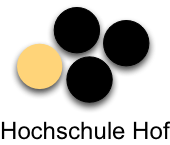
\includegraphics[height=0.05\textheight]{LogoGelb.png}}
\pagestyle{scrheadings}

\setcounter{secnumdepth}{3}
\setcounter{tocdepth}{3}
\renewcommand{\arraystretch}{1}

\parskip0.5\baselineskip plus 0.125\baselineskip minus 0.25\baselineskip
\parindent0em

% #################################################################

\def\SECH{S\kern-.075em \lower.5ex\hbox{E}\kern-0.05em CH\xspace}
\def\SEARCH{S\kern-.075em \lower.5ex\hbox{E}\kern-0.05em AR\kern-.075em \raise.5ex\hbox{C}\kern-0.05em H\xspace}

% #################################################################

%\automark[section]{chapter}

\titlehead{\begin{center}
\includegraphics[width=5cm]{fh_logo}\end{center}}
\title{
  \SEARCH--Tag EEXCESS \SECH--Browser \\[1em]
  Programmier Leitfaden\\
Spezifikation, Konstruktion
}

\author{Prof. Dr. Peter Stöhr \and Gottfried von Recum \and Alexander Pöhlmann \and Lothar Mödl \and Burak Erol \and Brian Mairhörmann \and Andreas Netsch \and Philipp Winterholler \and Andreas Ziemer}
\date{Version 0.4.1}

% #################################################################

\lstdefinelanguage{swift}
{
  morekeywords={
    func,if,then,else,for,in,while,do,switch,case,default,where,break,continue,fallthrough,return,
    typealias,struct,class,enum,protocol,var,func,let,get,set,willSet,didSet,inout,init,deinit,extension,
    subscript,prefix,operator,infix,postfix,precedence,associativity,left,right,none,convenience,dynamic,
    final,lazy,mutating,nonmutating,optional,override,required,static,unowned,safe,weak,internal,
    private,public,is,as,self,unsafe,dynamicType,true,false,nil,Type,Protocol,
  },
  morecomment=[l]{//}, % l is for line comment
  morecomment=[s]{/*}{*/}, % s is for start and end delimiter
  morestring=[b]" % defines that strings are enclosed in double quotes
}

\definecolor{keyword}{HTML}{BA2CA3}
\definecolor{string}{HTML}{D12F1B}
\definecolor{comment}{HTML}{008400}

\lstset{
  language=swift,
  basicstyle=\ttfamily,
  showstringspaces=false, % lets spaces in strings appear as real spaces
  columns=fixed,
  keepspaces=true,
  keywordstyle=\color{keyword},
  stringstyle=\color{string},
  commentstyle=\color{comment},
}

% #################################################################

\begin{document}
\maketitle
\pagenumbering{Roman}
\tableofcontents

%\newpage
\pagenumbering{arabic}

\part{Einleitung}
%\part{Einleitung}

\chapter{Übersicht}
\section{Abschnitt}
\subsection{Teilabschnitt}
\subsubsection{Unterteilabschnitt}
\paragraph{Paragraph}
\subparagraph{Unterparagraph}

\begin{enumerate}
     \item Eine
     \item kleine
     \item Aufzählung
\end{enumerate}

%\input{(Unter-)Datei}

%\part{Einleitung}

%\chapter{Übersicht}
%\section{Abschnitt}
%\subsection{Teilabschnitt}
%\subsubsection{Unterteilabschnitt}
%\paragraph{Paragraph}
%\subparagraph{Unterparagraph}

%\begin{enumerate}
%     \item Eine
%     \item kleine
%     \item Aufzählung
%\end{enumerate}
%\part{Einleitung}

\chapter{Programmlogik}
\section{Abschnitt}
\subsection{Teilabschnitt}
\subsubsection{Unterteilabschnitt}
\paragraph{Paragraph}
\subparagraph{Unterparagraph}

\begin{enumerate}
     \item Eine
     \item kleine
     \item Aufzählung
\end{enumerate}

Unter dem Punkt Programmlogik wird der ganze Anfrageprozess verstanden. Dieser beginnt beim Extrahieren von \lstinline|SearchModel|s bis zum Ausliefern der \lstinline|SearchResult|s und wird in folgende Komponenten gegliedert:

\begin{enumerate}
     \item \lstinline|SEARCHExtraction|
     \item \lstinline|QueryCreation|
     \item \lstinline|QueryResolution|
     \item \lstinline|Ranking|
\end{enumerate}

\begin{figure}[htb]
  \centering
  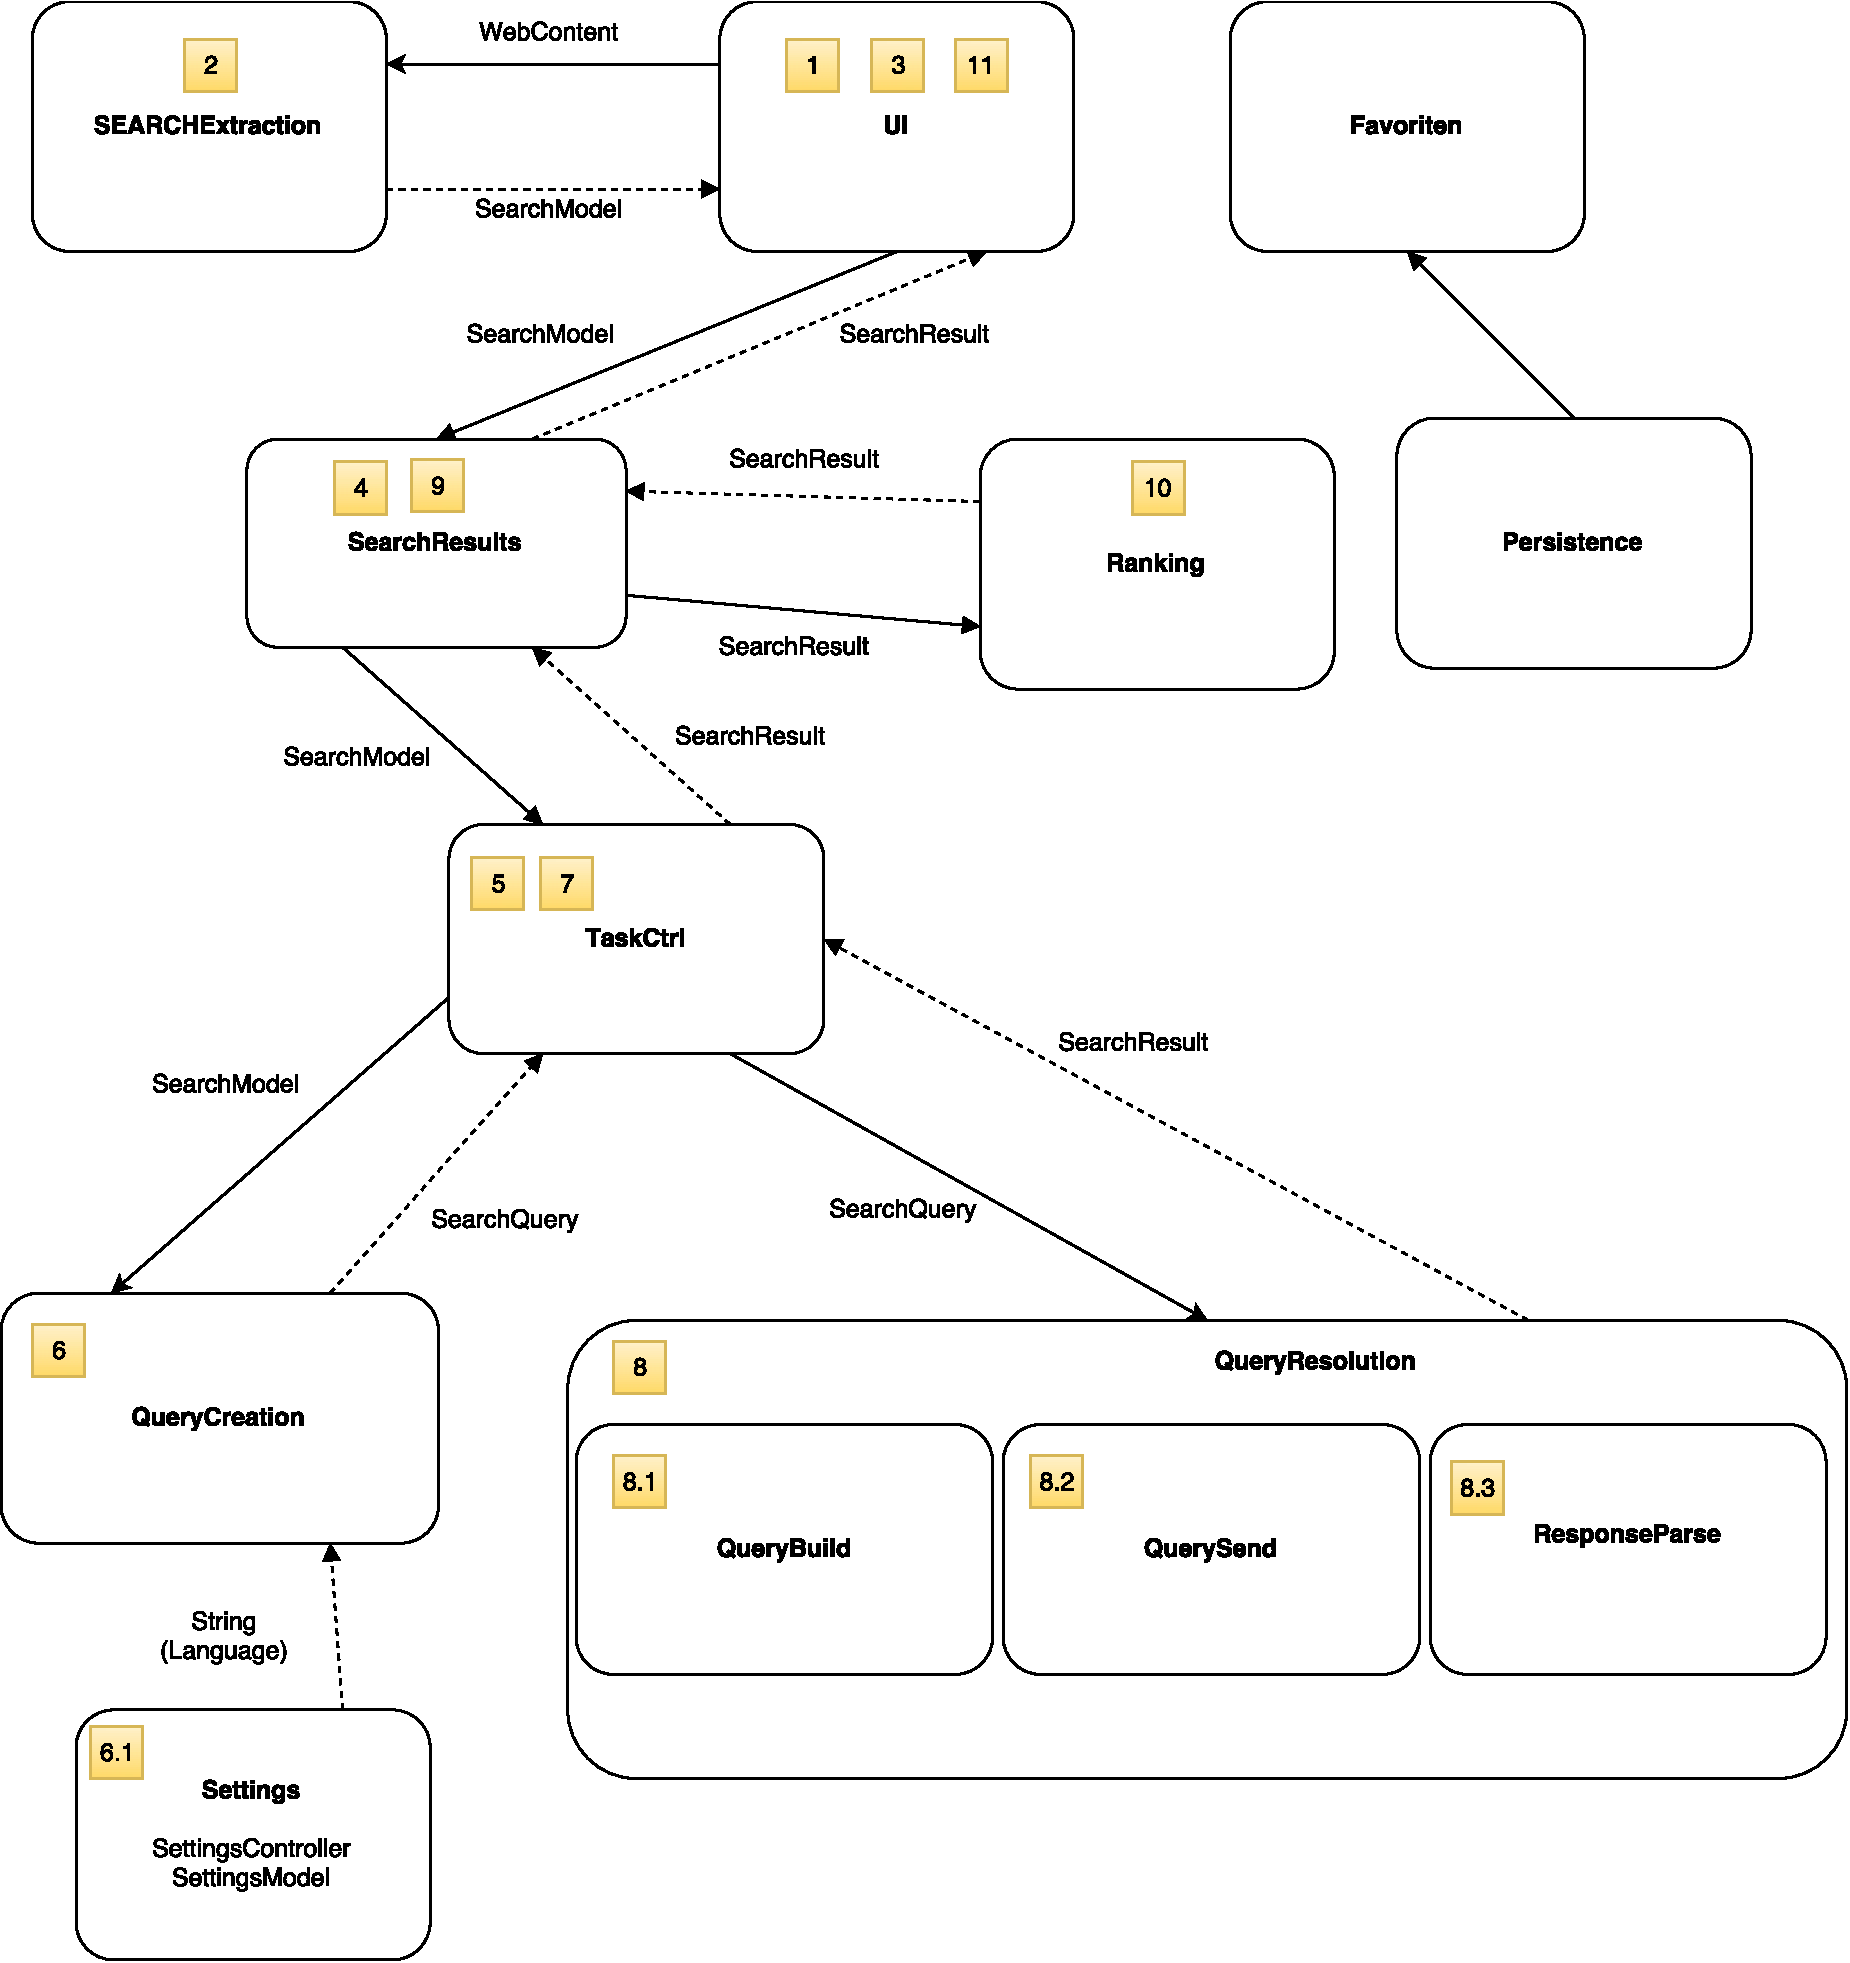
\includegraphics[width=0.6\textwidth]{Architektur}
  \caption{Übersicht des Kapitels Programmlogik}
\end{figure}



\part{Spezifikation}
%\part{Spezifikation}

\chapter{Kapitel}
\section{Abschnitt}
\subsection{Teilabschnitt}
\subsubsection{Unterteilabschnitt}
\paragraph{Paragraph}
\subparagraph{Unterparagraph}

\begin{enumerate}
     \item Eine
     \item kleine
     \item Aufzählung
\end{enumerate}

\part{Konstruktion}
%\part{Konstruktion}

\chapter*{Einleitung}
Die Konstruktion erklärt in einem HighLevel Ansatz die Implementierung des \SECH-Browsers. Das bedeutet wir betrachten aus der Vogelperspektive die Architektur und beobachten und beschreiben die Abläufe im Programm. Das ermöglicht einen guten Überblick über die Geschehnisse zu bekommen und die Vorgänge im Inneren nachvollziehen zu können. An entscheidenden Stellen sind weitere Erklärungen LowLevel im Programmcode als Kommentare eingefügt.

%\part{Konstruktion}

\chapter{User Interface}

%\part{Konstruktion}
%\chapter{User Interface}

\section{ViewController}
Der ViewController dient zur Steuerung der Funktionen welche direkt mit dem Interface zusammen gehören. Dazu gehören
IBActions welche von Buttons oder anderen Interkationsflächen angestoßen werden können, sowie Funktionen welche direkt mit diesen zusammenhängen, Beziehungsweise aus diesen resultieren. Der ViewController ist die zweite Schicht nach dem UI. Im
Folgenden werden die einzelnen Viewcontroller mit ihren jeweiligen Funktionen beschrieben.
Der Viewcontroller ist der Hauptviewcontroller für die normale Browseransicht mit der Adresszeile und dem WkWebView. Er verwaltet die Kopzeile mit Adresszeile sowie den Buttons für Vorwärts, Zurück, Lesezeichen, Lesezeichen hinzufügen, Reload, Sech-Tabelle sowie die Settings. Die datei Main.js welche aus dem Viewcontroller heraus aufgerufen wird, markiert alle gefundenen Search-Tags. Außerdem wird im Falle eines Klicks die Position sowie die id des Search-Tags übermittelt.
Der PopViewController ist zuständig für die Verwaltung eines neuen PopViews, beim klicken auf einen Searchtag. Er verwaltet die Anzeige des ausgewählten Searchlinks in einem neuen WkWebView sowie den Button für die Auswahl der verschiedenen Suchergebnisse zu einem Searchtag.
Der SearchTableViewController verwaltet die einzellnen Suchergebnisse zu einem Searchtag. Alle Ergebnisse werden sortiert in einer Tabelle mit Bild, Title und Link angezeigt.
Der Settingscontroller is für die verwaltung der Browsereinstellungen zuständig.
\subsection{ViewController}
\subsection{SearchTableViewController}
\subsection{PopViewController}
\subsection{SettingsController}
\subsection{main.js}
\subsection{readHead.js}

%\subsubsection{Unterteilabschnitt}
%\paragraph{Paragraph}
%\subparagraph{Unterparagraph}

\newpage
%\part{Konstruktion}
%\chapter{User Interface}

\section{Delegate}

Die Delegates im \SECH-Browser dienen zur Bereitstellung einer einheitlichen Struktur innerhalb des Programms. Von den einzelnen Delegate Klassen werden Funktionen zur Darstellung von Informationen oder interne Protokolle aufgerufen. Im \lstinline|WebViewDelegate| werden die Funktionen zur Validierung der Website mit Hilfe der JavaScript Dateien und die Extraktion der \SEARCH-Tags angestoßen.

Die \lstinline|readHead.js| enthält den Javascript Code zur Auslesen des Headbereiches einer HTML-Seite. In der Klasse \lstinline|FavTableDelegate| werden die Lesezeichen bereitgestellt. Der Benutzer hat die Möglichkeit ein ausgewähltes Lesezeichen auszuwählen und es sich im Browser anzeigen zulassen. Zusätzlich enhält die Klasse die Funktionen, um Lesezeichen bearbeiten und löschen zu können. Der SechTableDelegate enthält die Routine zum Darstellen von \SEARCH-Links aus der \SECH-Tabelle. 
\subsection{AppDelegate}
\subsection{WebViewDelegate}
\subsection{readHead.js}
\subsection{FavTableDelegate}
\subsection{SechTableDelegate}

%\subsubsection{Unterteilabschnitt}
%\paragraph{Paragraph}
%\subparagraph{Unterparagraph}

\newpage
%\part{Konstruktion}
%\chapter{User Interface}

\section{DataSource}
Die DataSources im \SECH-Browser dienen zur Bereitstellung der Daten in den Tabellen. Von den einzelnen Klassen werden jeweils Funktionen zum befüllen der einzelnen Zellen aufgerufen. In der Klasse FavTableDataSource werden zunächst alle gespeicherten Lesezeichen geladen, anschließend werden die einzelnen Zellen der Tabelle mit den Lesezeichen befüllt. Im SechTableDataSource werden alle \SEARCH-Tags die auf der Seite gefunden wurden in den Zellen der \SECH-Tabelle dargestellt. Zusätzliche befinden sich noch Funktionen zum Erweitern der \SEARCH-Tags in der Klasse.

\subsection{FavTableDataSource}
\subsection{SechTableDataSource}

%\subsubsection{Unterteilabschnitt}
%\paragraph{Paragraph}
%\subparagraph{Unterparagraph}


\newpage
%\part{Konstruktion}
%\chapter{User Interface}

\section{Components}

In den Components werden die spezifischen Zellen für die Lesezeichen-Tabelle und Search-Tag-Tabelle modelliert, die in den jeweiligen Delegates verwendet werden. Weiterhin ist in Components die Validierung für die AddressBar definiert, welche die Eingaben in der Suchleiste überprüft und verwaltet.

\newpage
%\part{Konstruktion}
%\chapter{User Interface}
%\section{Packages}

\subsection{Persistence}
Im Persistence-Package befinden sich Models die für eine persistente Speicherung gedacht sind. Das \lstinline|FavouritesModel| stellt einerseits das nötige Model, andererseits die Funktion für das Speichern von Lesezeichen zur Verfügung.
\newpage
%\part{Konstruktion}
%\chapter{User Interface}

\section{WebContent}

Der \lstinline|WebContent| stellt die Schnittstelle zwischen dem UI und der SearchExtraction dar. Er beinhaltet HTML-Code, in Form eines Strings, sowie die URL, von welcher der HTML-Code stammt. Der HTML-Code ist in den Head und den Body der Website aufgeteilt.\newline
Aus dem \lstinline|WebContent| wird in der SearchExtraction ein \lstinline|SearchModel| erzeugt.

%\subsection{Teilabschnitt}
%\subsubsection{Unterteilabschnitt}
%\paragraph{Paragraph}
%\subparagraph{Unterparagraph}



%\part{Konstruktion}

\chapter{Programmlogik}

Unter dem Punkt Programmlogik wird der ganze Anfrageprozess verstanden. Dieser reicht vom Extrahieren von \lstinline|SearchModel|s bis hin zum Ausliefern der \lstinline|SearchResult|s stützt sich auf folgende wichtige Komponenten:

\begin{enumerate}
     \item \lstinline|SEARCHExtraction|
     \item \lstinline|QueryCreation|
     \item \lstinline|QueryResolution|
     \item \lstinline|Ranking|
\end{enumerate}

\begin{figure}[htb]
  \centering
  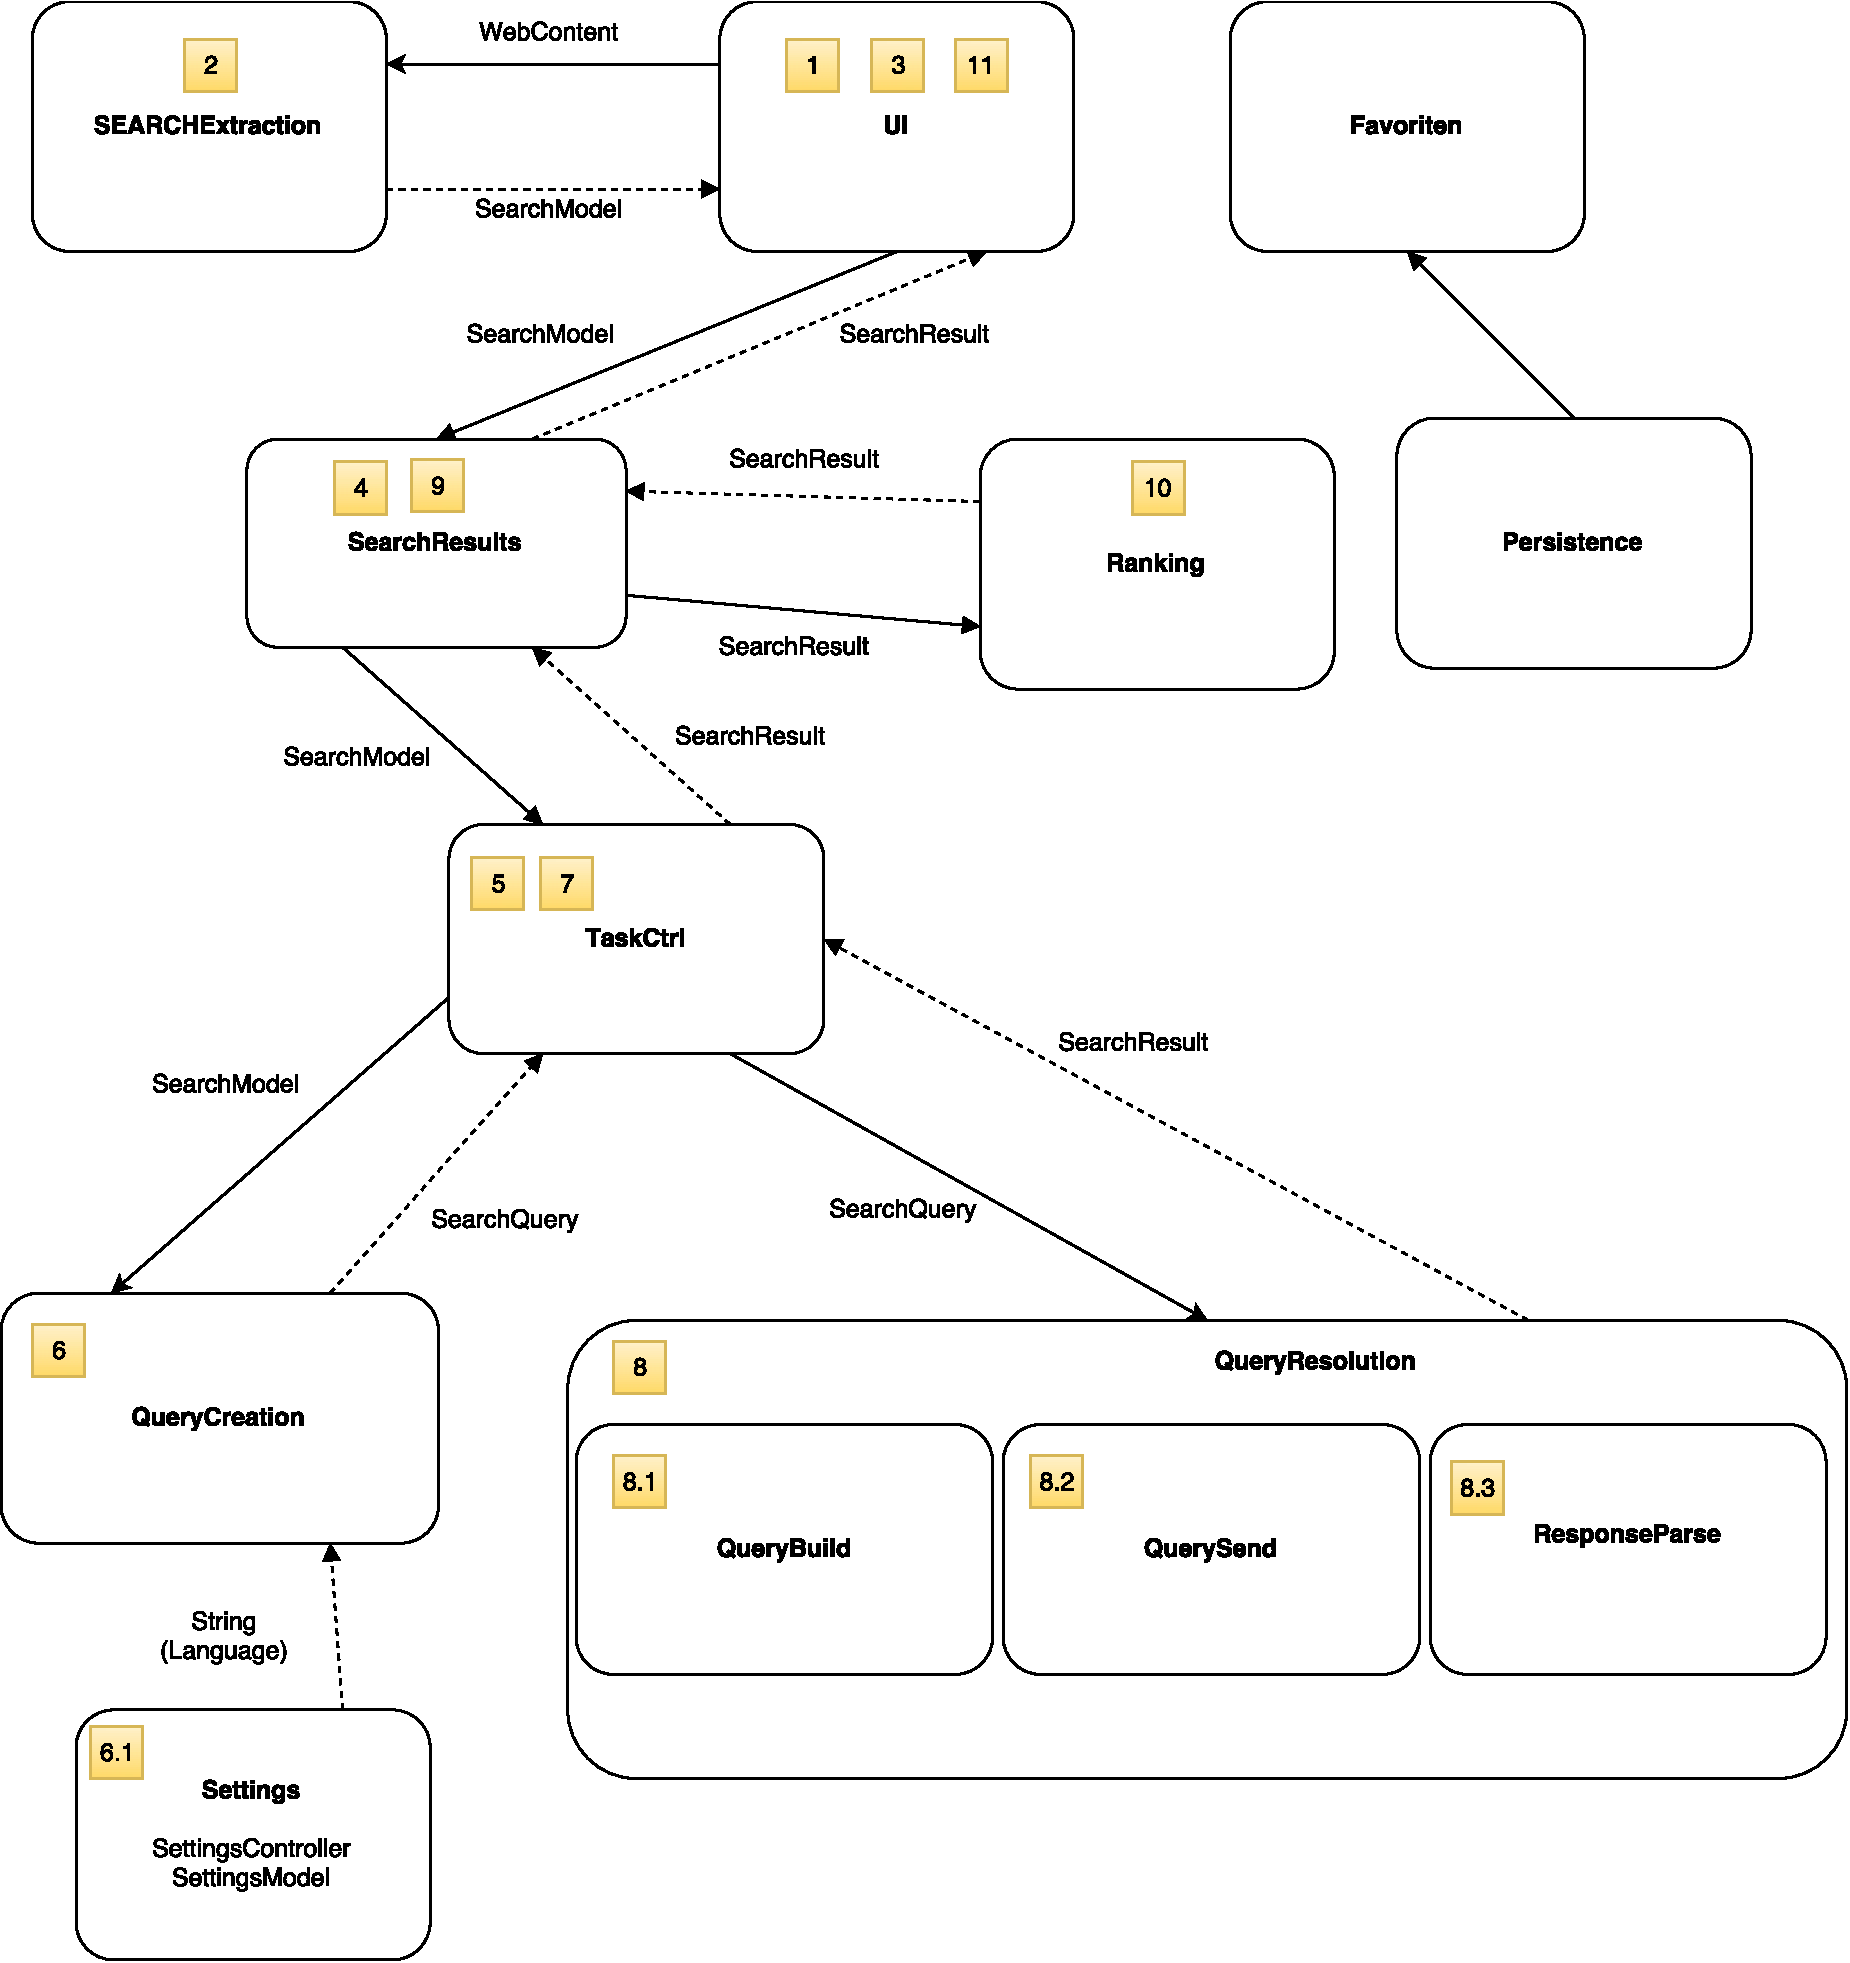
\includegraphics[width=\textwidth]{Architektur}
  \caption{Übersicht des Kapitels Programmlogik}
\end{figure}

Im Folgenden werden alle Teile der Programmlogik beschrieben.

%\part{Konstruktion}
%\chapter{Programmlogik}

\section{TaskCtrl}

Der \lstinline|TaskCtrl| ist einer der wichtigsten Elemente bei der Kommunikation zwischen der Oberfläche und dem Abrufen der Daten aus dem Internet. Er bestimmt mit Hilfe der vom Nutzer getroffenen Einstellungen an welche Suchmaschine die Anfrage geschickt wird. Die Einstellungen werden durch das \lstinline|Settings.bundle| definiert und können durch die Klasse \lstinline|SettingsManager| abgerufen werden. 

Der \lstinline|TaskCtrl| wird von der Klasse \lstinline|SearchResults| initialisiert und aufgerufen. Zuerst werden unter Verwendung der Klasse \lstinline|QueryCreationCtrl| Daten in einem allgemeingültigen Format für die Suchanfragen erstellt. Diese Daten werden daran anschließend von den jeweiligen \lstinline|QueryBuildern| (\lstinline|EEXCESSJSONBuilder|, \lstinline|DuckDuckGoURLBuilder| und \lstinline|FarooURLBuilder|) in das für die jeweilige Suchmaschine passende Datenformat umgewandelt. Die Suchanfragen werden asynchron durch die entsprechenden \verb|ConnectionCtrl| (\lstinline|JSONConnectionCtrl| und \lstinline|URLConnectionCtrl|) versendet. Bei erfolgreicher Suche und nach erfolgreichem Parsen der Ergebnisse werden diese dann mit Aufruf der Methode \lstinline|setRecommendation(|\lstinline|status:String,| \lstinline|message:String,| \lstinline|result:SearchResult)| an den Aufrufer, die Klasse \lstinline|SearchResults|, zurückgegeben. Diese speichert die Suchergebnisse in einem Cache zwischen. Der \lstinline|TaskCtrl| wird nur aufgerufen, falls zu dem jeweiligen \SEARCH-Tag noch keine Ergebnisse im Cache vorhanden sind. 

%\subsection{Teilabschnitt}
%\subsubsection{Unterteilabschnitt}
%\paragraph{Paragraph}
%\subparagraph{Unterparagraph}

%\begin{sloppy}

%\part{Konstruktion}
%\chapter{Programmlogik}

\section{SEARCHExtraction}

\subsection{SearchManager}
\subsection{RegexForSEARCH}

%\subsubsection{Unterteilabschnitt}
%\paragraph{Paragraph}
%\subparagraph{Unterparagraph}

%\part{Konstruktion}
%\chapter{Programmlogik}

\section{SEARCHModels}
Das SearchModels stellt die Schnittstelle zwischen der SearchExtraction und dem TaskController dar. Von der SearchExtraction erzeugt beinhaltet ein SearchModels-Objekt eine Sammlung von SearchModel-Objekten erzeugt aus einer Website. In einem SearchModel-Objekt werden Search-Tag-Links mit der zugehörigen Search-Tag-Section/-Head und Filtern gespeichert.\newline
Zur globalen Identifikation wird in einem SearchModel die Url der Website von der es kommt gesetzt. Um ein SearchModel innerhalb einer Seite zu finden wir der Index gesetzt.

%\subsection{Teilabschnitt}
%\subsubsection{Unterteilabschnitt}
%\paragraph{Paragraph}
%\subparagraph{Unterparagraph}

%\part{Konstruktion}
%\chapter{Programmlogik}

\section{QueryCreation}

\begin{figure}[htb]
   \centering
  	\includegraphics[width=0.4\textwidth]{QueryCreation}
  	\caption{Aufbau des Moduls \lstinline|QueryCreation|}
\end{figure}
\lstinline|QueryCreation| generiert aus den Suchwörtern (\lstinline|SearchModel|) und den Geräte- und App-Einstellungen ein allgemeines Anfrageformat. Dieses Anfrageformat wird in \lstinline|QueryResolution| zu einem für jede Suchmaschine spezifischen Suchformat umgewandelt.

\subsection{QueryCreationCtrl}

%\subsubsection{Unterteilabschnitt}
%\paragraph{Paragraph}
%\subparagraph{Unterparagraph}

%%\part{Konstruktion}
%\chapter{Programmlogik}

\section{SearchQuerys}
%\part{Konstruktion}
%\chapter{Programmlogik}

\section{QueryResolution}

\begin{figure}[htb]
  	\includegraphics[width=\textwidth]{qr_querysend.png}
  	\caption{Aufbau des Moduls QueryResolution}
	\label{fig:Aufbau des Moduls QueryResolution}
\end{figure}

%\part{Konstruktion}
%\chapter{Programmlogik}
%\section{QueryResolution}

\subsection{JSONData}

%\paragraph{Paragraph}
%\subparagraph{Unterparagraph}

\newpage
%\part{Konstruktion}
%\chapter{Programmlogik}
%\section{QueryResolution}

\subsection{QueryBuild}

Das Modul QueryBuild liefert den größten Teil der Intelligenz im Modul QueryResolution. Die Aufgaben des Moduls sind es, die ConnectionController in QuerySend zu konfigurieren, die Query in das suchmaschinenspezifische Anfrageformat umzuwandeln und dem ConnectionController den Parser für die Antwort zu geben.

Es gibt für jede Suchmaschine eine Implementation der Spezifikation AbstractBuilder, welche durch die Spezifikationen URLAbstractBuilder und JSONAbstractBuilder erweitert wird.

\subsubsection{AbstractBuilder}
\subsubsection{AbstractJSONBuilder}
\subsubsection{AbstractURLBuilder}
\subsubsection{EexcessJSONBuilder}
\subsubsection{FarooURLBuilder}
\subsubsection{DuckDuckGoURLBuilder}
\subsubsection{EEXCESSOrigin}

%\paragraph{Paragraph}
%\subparagraph{Unterparagraph}

\newpage
%\part{Konstruktion}
%\chapter{Programmlogik}
%\section{QueryResolution}

\subsection{QuerySend}

\begin{figure}[htb]
	\centering
  	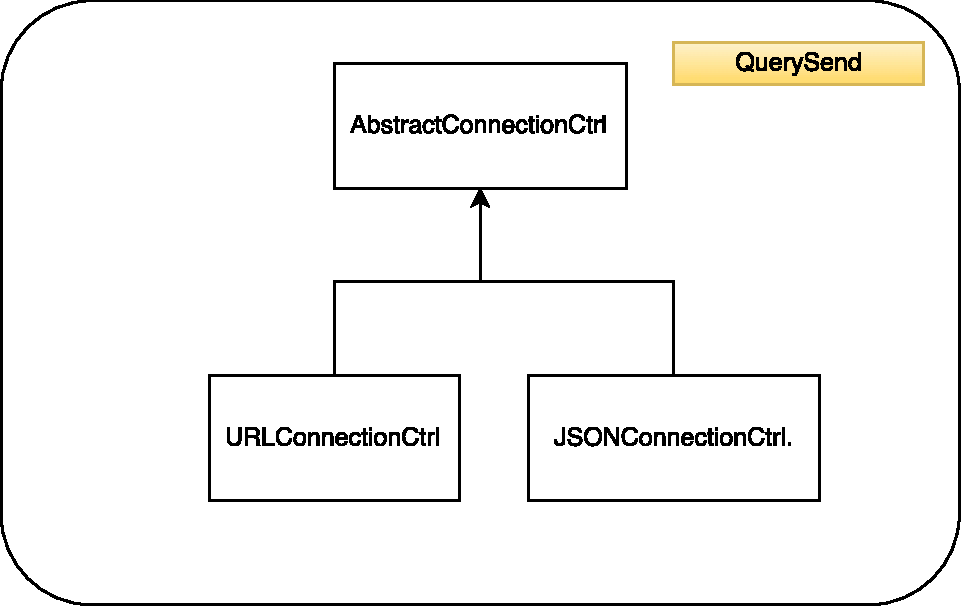
\includegraphics[width=0.8\textwidth]{qr_querysend}
  	\caption{Aufbau des Moduls \lstinline|QuerySend|}
\end{figure}

Im Modul \lstinline|QuerySend| befinden sich die \lstinline|ConnectionController|, die für das Versenden der Anfrage zuständig sind. Sie werden mithilfe von \lstinline|QueryBuild| konfiguriert und erhalten den Parser (\lstinline|ResponseParse|). Vor dem Weiterreichen an den \lstinline|TaskController|, wird durch den Parser noch von NSData zu \lstinline|SearchResult| umgewandelt.
\newpage
%\part{Konstruktion}
%\chapter{Programmlogik}
%\section{QueryResolution}

\subsection{ResponseParse}
\begin{figure}[htb]
	\centering
		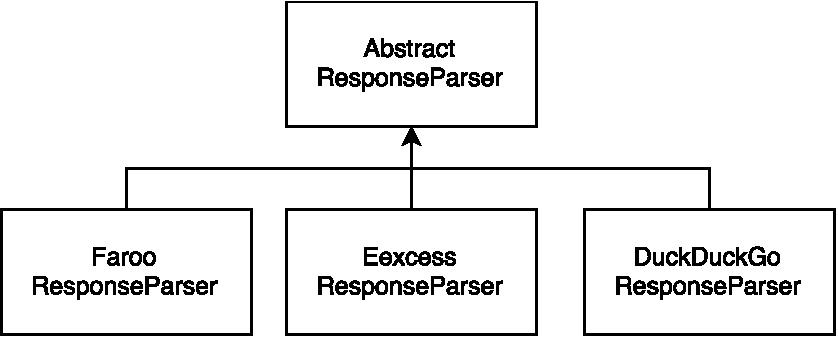
\includegraphics[]{response_parser}
		\caption{Aufbau des Moduls ResponseParse}
		\label{fig:Aufbau des Moduls ResponseParse}
\end{figure}
Der \lstinline|ResponeParser| ist für das Parsen der Antworten der Suchmaschinen in ein allgemeines Format.
Dabei wird in der aktuellen Version zwischen drei Parsern unterschieden.
\subparagraph{FarooResponseParser}
Hier werden die Antworten von Faroo verarbeitet.
\subparagraph{DuckDuckGoResponseParser}
Hier werden die Antworten von DuckDuckGO verarbeitet.
\subparagraph{EexcessResponseParser}
Hier werden die Antworten von Eexcess verarbeitet.
\subparagraph{AbstractResponseParser}
Der \lstinline|AbstractResponseParser| spezifiziert wie die untergeordneten \lstinline|ResponeParser| implementiert werden.

%\paragraph{Paragraph}
%\subparagraph{Unterparagraph}




%\paragraph{Paragraph}
%\subparagraph{Unterparagraph}

%\part{Konstruktion}
%\chapter{Programmlogik}

\section{SearchResults}
\begin{figure}[htb]
  \centering
  \includegraphics[width=0.4\textwidth]{SearchResults2}
  \caption{Ablaufmöglichkeiten im \lstinline|SearchResults|}
\end{figure}

\lstinline|SEARCHResults| ist ein Container, der für ein Suchwort die Suchergebnisse speichert.
Der Container ist in der Lage, bei fehlenden Suchergebnissen Suchanfragen abzuschicken und informiert mit dem Observer, ob neue Suchergebnisse von der Suchmaschine gekommen sind. Der Observer wird im \lstinline|PopViewController| registriert und ist somit in der Lage auf neue Suchergebnisse zu reagieren. 
%\subsection{Teilabschnitt}
%\subsubsection{Unterteilabschnitt}
%\paragraph{Paragraph}
%\subparagraph{Unterparagraph}

\pagebreak
%\part{Konstruktion}
%\chapter{Programmlogik}

\section{Ranking}
\subsection{Rules}
\subsection{SearchRules}
\subsection{RankingPersistence}
\subsubsection{PersistenceController}
\subsubsection{RankingDataObject}
\subsubsection{RankingDataObjectPersistency}

%\paragraph{Paragraph}
%\subparagraph{Unterparagraph}

\section{SettingsModel}
Im SettingsModel werden die verschiedenen Einstellungen für den Browser gespeichert.
Der Nutzer kann diese über das Einstellungsmenü des Geräts ändern.

\paragraph{Einstellungen}  

Die Einstellungen sind in drei verschiedene Kategorien eingeteilt.
\begin{itemize}  
     \item Suchmaschinen  
     \item Nutzerprofil
     \item Browsereinstellungen
\end{itemize}

\subparagraph{Suchmaschinen}  

Hier kann der Nutzer die verschiedenen Suchmaschinen einstellen, die für die SearchTags verwendet werden sollen.
Dabei kann entweder jede Suchmaschine einzeln gewählt werden, oder den Empfehlungen des Autors gefolgt werden.
Zur Auswahl stehen:
\begin{itemize}  
     \item DuckDuckGo
     \item Eexcess
     \item Faroo  
\end{itemize}
Sobald eine Suchmaschine gewählt wurde, werden die Empfehlungen des Autors ignoriert.

\subparagraph{Nutzerprofil}  
Hier können die Nutzerdaten angegeben werden.
Davon wird bisher nur die Sprach verwendet.
Einstellungsmöglichkeiten:
\begin{itemize}  
     \item Name  
     \item Alter  
     \item Stadt
     \item Land
     \item Sprache
\end{itemize}

\subparagraph{Startseite}  
Hier kann die Startseite des Browser festgelegt werden.
Die hier gesetzte Seite wird nocht nicht im Browser als Startseite übernommen.



%\newpage
\listoffigures
\listoftables
\end{document}
